\chapter{Chapter 1 Title}\label{chap1}
%\fixchapterheading % Use this if section follows chapter immediately

Text

\section{Section Title}  % level 2
Text 
   \begin{table}[b]
    \caption{Experimental values for toe parameters while perching.}
    \label{tab:footData}
    \begin{center}
    \begin{tabular}{c|c|c|}
      \cline{2-3}
      % after \\: \hline or \cline{col1-col2} \cline{col3-col4} ...
      {} & \textbf{33\,mm Perch} & \textbf{49\,mm Perch} \\\hline
      \multicolumn{1}{|c|}{\textbf{$\delta$}} & 37\,mm & 31\,mm \\
      \multicolumn{1}{|c|}{\textbf{$\theta_1$}} & $(62^\circ+52^\circ)/2=57^\circ$ & $(56^\circ+39^\circ)/2=47^\circ$ \\
      \multicolumn{1}{|c|}{\textbf{$\theta_2$}} & $(60^\circ+66^\circ)/2=63^\circ$ & $(51^\circ+53^\circ)/2=52^\circ$ \\
      \multicolumn{1}{|c|}{\textbf{$\theta_3$}} & $(66^\circ+71^\circ)/2=68^\circ$ & $(57^\circ+61^\circ)/2=59^\circ$ \\
      \hline
    \end{tabular}
    \end{center}
   \end{table}
Text 
   \begin{figure}[t]
      \centering
      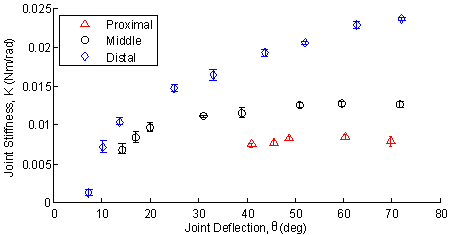
\includegraphics[width=.7\textwidth]{chap1img/jointDeflection4.pdf}
      \caption[Joint stiffness as a function of deflection]{Joint stiffness as a function of deflection. Values are calculated using the mean joint deflections reported in Table \ref{tab:deflect}. Error bars show the range of K values possible with all permutations of $\pm\sigma$ in joint deflection. Stiffness is nonlinearly related to deflection and increases as the toe deflects further.}
      \label{fig:jointDeflect}
   \end{figure}

\subsection{Subsection Title} %level 3
Text  